% Preamble %%%%%%%%%%%%%%%%%%%%%%%%%%%%%%%%%%%%%%%%%%%%%%%
\documentclass{thesis}
%%%%%%%%%%%%%%%%%%%%%%%%%%%%%%%%%%%%%%%%%%%%%%%%%%%%%%%%%%
%\usepackage{setspace}
%\usepackage[xindy]{glossaries}
%\newglossarystyle{customstyle}{%
%% put the glossary in the itemize environment:
%\renewenvironment{theglossary}{}{}%
%% have nothing after \begin{theglossary}:
%\renewcommand*{\glossaryheader}{}%
%% have nothing between glossary groups:
%\renewcommand*{\glsgroupheading}[1]{}%
%\renewcommand*{\glsgroupskip}{}%
%% set how each entry should appear:
%\renewcommand*{\glossaryentryfield}[5]{%
%%\item[] % bullet point
%\glstarget{##1}{##2}% the entry name
%\dotfill% the symbol in brackets
%\space ##3 \\% the number list in square brackets
%}%
%% set how sub-entries appear:
%\renewcommand*{\glossarysubentryfield}[6]{%
%\glossaryentryfield{##2}{##3}{##4}{##5}{##6}}%
%}
%\makeglossaries
%\glossarystyle{customstyle}
%\def\glossaryname{واژه نامه}
%\newglossaryentry{گروه}{name=گروه,
%description={Group }}
%\newglossaryentry{چنبره}{name=چنبره,
%description={Torus }}
%\newglossaryentry{پردازشگر}{name=پردازشگر,
%description={Processor }}
%\newglossaryentry{کلاف}{name=کلاف,
%description={Bundle }}
%\newglossaryentry{شما}{name=شما,
%description={Scheme }}
%\newglossaryentry{رایانه}{name=رایانه,
%description={Computer }}
%\newglossaryentry{موسیقی}{name=موسیقی,
%description={Music }}
%\newglossaryentry{شعر}{name=شعر,
%description={Poem }}
%\newglossaryentry{زی‌پرشین}{name=زی‌پرشین,
%description={\XePersian }}
%\newglossaryentry{واژه‌نامه}{name=واژه‌نامه,
%description={Glossary }}
%\newglossaryentry{آنتن}{name=آنتن,
%description={Antenna }}
%%%%%%%%%%%%%%%%%%%%%%%%%%%%%%%%%%%%%%%%%%%%%%%%%%%%%%%%%%
\usepackage[colorlinks=true]{hyperref}
\usepackage{hyperref}
\hypersetup{
  linkcolor  = black,
  citecolor  = black,
  urlcolor   = black,
  colorlinks = true,
}
\usepackage{amssymb}
\usepackage{xepersian}
\settextfont[Scale=1]{XBNiloofar}
% Title page %%%%%%%%%%%%%%%%%%%%%%%%%%%%%%%%%%%%%%%%%%%%%
\begin{document}
\logo{
\includegraphics{logo}}
\date{
۴ تیر ۱۳۹۶
}
\title{
تحلیلی بر عملکرد حافظه مشترک تحت بارهای کاری چند منظوره در پردازنده‌های گرافیکی
}
\author{
پارسوآ خورسند رحیم‌زاده
}
\university{%
دانشگاه صنعتی شریف
\\
دانشکده مهندسی کامپیوتر
}
\subject{%
مهندسی نرم‌افزار
}
\supervisor{
دکتر حمید سربازی آزاد
}
\frontmatter \makethesistitle \pagestyle{empty} \baselineskip1.2\baselineskip
% Abstract %%%%%%%%%%%%%%%%%%%%%%%%%%%%%%%%%%%%%%%%%%%%%%%
\begin{abstract}
{%
پردازنده‌های گرافیکی عام‌منظوره، حافظه مشترک، کارایی، زمان دسترسی
}
{%
در پردازنده‌های گرافیکی روی هر چند‌پردازنده جریانی
%\newglossaryentry{sm}{
%name=چند‌پردازنده جریانی,
%description={Streaming Multiprocessor}
%}
یک واحد حافظه اختصاصی برای نگهداری داده‌های مربوط به فضای آدرس‌دهی مشترک 
%\newglossaryentry{sharedaddressspace}{
%name=فضای‌آدرس‌دهی مشترک,
%description={Shared Address Space}
%}
ریسمان‌های در حال اجرا تعبیه شده‌است. فضای این حافظه به بلوک‌های هر چندپردازنده
به
طور
جداگانه تخصیص می‌یابد و میان ریسمان‌های
%\newglossaryentry{thread}{
%name=ریسمان,
%description={Thread}
%}
 هر بلوک به طور مشترک استفاده می‌شود.

حافظه مشترک
%\newglossaryentry{sharedmemory}{
%name=حافظه مشترک,
%description={Shared Memory}
%}
 به برنامه‌نویس اجازه می‌دهد تا اطلاعات مورد نیاز برای اجرای هر بلوک از
ریسه‌های برنامه را روی چندپردازنده‌ جریانی شامل آن‌ها ذخیره کند. حافظه مشترک به
دلیل ظرفیت و در نتیجه مساحت کم و نیز قرار گرفتن روی تراشه چند‌پردازنده زمان
دسترسی بسیار پایینی (در حد چند کلاک) دارد. به این ترتیب برنامه‌نویس می‌تواند
بخشی از داده را که احتمال می‌دهد قرار است در باز زمانی فعلی با نرخ بالا مورد
دسترسی قرار گیرد را روی این حافظه بارگذاری
%\newglossaryentry{upload}{
%name=بارگذاری,
%description={Upload}
%}
  کند تا دسترسی به آن با سربار کم امکان‌پذیر باشد. 
  
  
  در نسل‌های اولیه پردازنده‌های گرافیکی، حافظه‌مشترک به عنوان راه‌حلی برای
مدیریت پیچیدگی‌های ناشی از زمان دسترسی غیر‌قابل پیش‌بینی حافظه‌ اصلی مورد
پیاده‌سازی قرار گرفت. چنین رویکردی در کاربرد‌های گرافیکی که نیاز به تضمین نرخ
فریم
%\newglossaryentry{framerate}{
%name=نرخ فریم,
%description={Frame Rate}
%}
ثابتی وجود دارد از توجیه‌پذیری بالایی برخوردار است.

در ادامه نتایج تحلیل روی عملکرد و میزان کاربرد حافظه مشترک در بارهای کاری
%\newglossaryentry{workload}{
%name=بار کاری,
%description={Workload}
%}
محاسباتی ارائه می‌شود و در نهایت راهکار‌هایی برای بهبود کارایی 
%\newglossaryentry{performance}{
%name=کارایی,
%description={Performance}
%}
این مدل حافظه پیشنهاد می‌گردد
.
}
\end{abstract}
% Appendix %%%%%%%%%%%%%%%%%%%%%%%%%%%%%%%%%%%%%%%%%%%%%%%
\pagestyle{plain} \pagenumbering{tartibi}
\tableofcontents
\listoffigures
\cleardoublepage
% Introduction %%%%%%%%%%%%%%%%%%%%%%%%%%%%%%%%%%%%%%%%%%%
\mainmatter \pagestyle{headings}\baselineskip1.1\baselineskip

\chapter{%
مقدمه
}

بر اساس قانون مور
\LTRfootnote{
Moore's Law
}
چگالی ترانزیستور‌های تراشه‌های نیمه‌رسانا
\LTRfootnote{
Semiconductor
}
پس از گذشته به طور تقریبی هر هجدهماه، دو‌ برابر می‌شود. در نتیجه می‌توان گفت که
پردازنده‌ها کوچکتر‌، چگال‌تر و قدرتمند‌تر می‌شوند. بر اساس این قانون حداکثر
فرکانس‌ کاری پردازنده‌ها نیز قابل افزایش به نظر می‌رسد. اما به دلایل گوناگون
روند افزایش  فرکانس کاری پردازنده‌ها در سال‌های اخیر با کندی مواجه شده است.
با ادامه روند افزایش فرکانس پردازنده‌ها، پیش‌بینی می‌شد که تا حوالی سال ۲۰۰۵
میلادی چگالی توان تراشه‌ها به سطح راکتور‌های هسته‌ای برسد.

\begin{figure}[h]
\centering
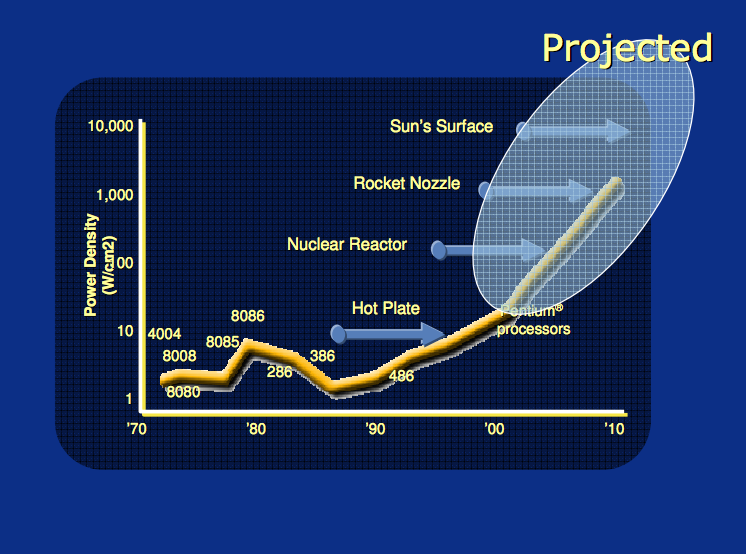
\includegraphics[width=\textwidth]{./pics/1}
\caption{پیش‌بینی رشد چگالی توان پردازنده‌ها}
\end{figure}

\section{پردازنده‌های چندهسته‌ای}

علی‌رغم پیشرفت‌ چشمگیر قدرت محساباتی سخت‌افزار‌ها و نیز نزدیک‌ شدن به موانع
عملی و فیزیکی برای افزایش فرکانس‌کاری آن‌ها، نیاز به بهبود عملکرد 
\LTRfootnote{Performance}
تراشه‌ها برای پشتیبانی از نیازمندی‌های جدید نرم‌افزار (به طور خاص رابط کاربری
گرافیکی) و نیز انجام‌ها پردازش رو مجموعه‌داده‌های
\LTRfootnote{Dataset}
 گسترده احساس می‌شد. 
در حدود سال ۲۰۰۰ میلادی اینتل
با معرفی پردازنده‌های با معماری
NetBurst
انتظار دستیابی به فرکانس کاری
\lr{10Ghz}
را داشت اما در عمل به علت مشکلات گرما و توان مصرفی عملیات این چیپ‌ها فرکانس‌های
بالای
\lr{4Ghz}
بدون استفاده از سیستم‌های خنک‌کننده بزرگ و پیچیده
(معمولا مبتنی بر آب)
امکان‌پذیر نبود.

 در این میان ایده
  پردازنده‌های چندهسته‌ای به عنوان راه‌حلی
برای افزایش کارایی ارائه شد. با توجه به اینکه در این فرکانس کاری پردازنده
افزایش نمیابد، پارامتر‌های توان مصرفی و در نتیجه چگالی توان نیز تغییر شگرفی
نمی‌کنند ولی چنانچه محسابات را بتوان به قسمت‌هایی با قابلیت موازی‌سازی تقسیم
کرد می‌توان زمان اجرا را به طور قابل توجهی کاهش داد. میزان 
ایده‌آل
بهبود عملکرد محاسبه
در این حالت از قانون امدال
\LTRfootnote{Amdahl's law}
پیروی می‌کند.

 لازم به ذکر است که تا قبل از ظهور پردازنده‌های چندهسته‌ای با 
تعریف امروزی گاها
از
چند پردازنده‌ی مرکزی مستقل برای انجام محاسبت استفاده می‌شد.  در این معماری هر
پردازنده عملا یک چیپ جداگانه بود که به واسطه یک باس
\LTRfootnote{Bus}
مشترک به مادربورد و حافظه اصلی متصل می‌شد. این استقلال فیزیکی پردازنده‌ها
مشکلات مختلفی ایجاد می‌کرد که در معماری‌های جدیدتر با قراردادن چند هسته
\LTRfootnote{Core}
 پردازشی
داخل یک تراشه 
تا حدی برطرف شده است.

\section{
پردازنده‌های گرافیکی
}

تاریخچه پردازنده‌های گرافیکی به حدود سال‌های دهه ۷۰ میلادی بازمی‌گردد، زمانی که
واحد‌های سخت‌افزاری جداگانه برای بهبود عملکرد رایانه در اجرای باز‌ی‌ها استفاده
می‌شد. نسخه‌های اولیه چنین پردازنده‌هایی چیزی عملا گسترش جزیی معماری
پردازنده‌های
برداری
\LTRfootnote{Vector Processor}
برای کاربرد‌های گرافیکی بودند. در چنین پردازنده‌هایی که به طور خاص برای پردازش
سیگنال
و
داده‌های
در
قالب ماتریس و آرایه طراحی شده بودند، تعداد زیادی واحد ریاضیاتی
\LTRfootnote{Arithmetic Logic Unit}
 به طور
همزمان دستورات یکسانی را روی قسمت‌های مختلف داده ورودی اجرا می‌کردند. این
رویکرد که به اصطلاح مدل
\textit{دستور واحد و داده‌های متفاوت}
\LTRfootnote{Single Instruction, Multiple Data (SIMD)}
نامیده می‌شود
به طور خاص در محاسبات جبر خطی
\LTRfootnote{Linear Algebra}
سودمند است.

پردازنده‌های گرافیکی در ابتدا سخت‌افزار‌هایی با عملکرد ثابت
\LTRfootnote{Fixed-Function}
بودند و امکان برنامه‌پدیری 
\LTRfootnote{Programmability}
نداشتند.
با افزایش قدرت پردازنده‌های گرافیکی طی نسل‌های متمادی و آشکار شدن پتانسیل این
روش پردازش برای کاربرد‌هایی خارج از حوزه گرافیک و بازی‌های رایانه‌ای، به مرور
زمان قابلیت برنامه‌پذیری نسبی به این سخت‌افزار‌ها اضافه شد و امروزه واسط‌های
نرم‌افزاری سطح بالای قدرتمندی مانند کودا
\LTRfootnote{CUDA: Compute Unified Device Architecture}
 توسعه داده
توسط شرکت
Nvidia
و
OpenCL
برای منظور پیاده‌سازی برنامه‌های موازی عام‌منظوره روی این تراشه‌ها 
در دسترس هستند.

یک پردازنده گرافیکی به طور معمول متشکل است از تعدادی چند‌پردازنده
\LTRfootnote{Multiprocessor}
که به صورت موازی دستورات (نه لزوما یکسان) را اجرا می‌کنند. به عنوان مثال
پردازنده گرافیکی
\lr{Nvidia Tesla K40}
بر پایه معماری
\lr{Kepler}
از ۱۵ چند‌پردازنده‌ جریانی
\LTRfootnote{Streaming Multiprocessor (SM)}
هر کدام با 
۱۹۲
هسته پردازشی عدد طبیعی
\LTRfootnote{Integer}
، ۶۴ هسته پردازشی عدد ممیزدار
\LTRfootnote{Floating Point}
 و ۳۲ واحد انتقال داده
\LTRfootnote{Load/Store Unit}
تشکیل یافته است.
این هسته‌ها به ۱۲ مجموعه 
\textit{دستور واحد و داده‌های متفاوت}
تقسیم می‌شود که هریک می‌توانند به طور مستقل دستور
واحدی‌ را روی داده ورودی خود اجرا کند
.
همچنین هر
چند‌پردازنده‌ جریانی
دارای یک واحد حافظه مشترک
\LTRfootnote{Shared Memory}
میان تمام هسته‌های پردازشی خود است که برای ذخیره داده‌های مورد نیاز در پردازش
فعلی و عدم نیاز به بارگیری
\LTRfootnote{Fetch}
آن‌ها از حافظه اصلی  در حین اجرا استفاده می‌شود.

در چنین معماری که با نام
\textit{دستور واحد و ریسه‌های متعدد}
\LTRfootnote{Single Instruction, Multiple Threads (SIMT)}
بازاریابی می‌شود تعداد زیادی
ریسه
به طور همزمان روند‌های اجرایی متفاوتی را روی داده اعمال می‌کنند.
یک پردازنده گرافیکی با معماری کپلر می‌تواند
۲۸۸۰
ریسه را به صورت موازی اجرا کند.

\begin{figure}[h]
\centering
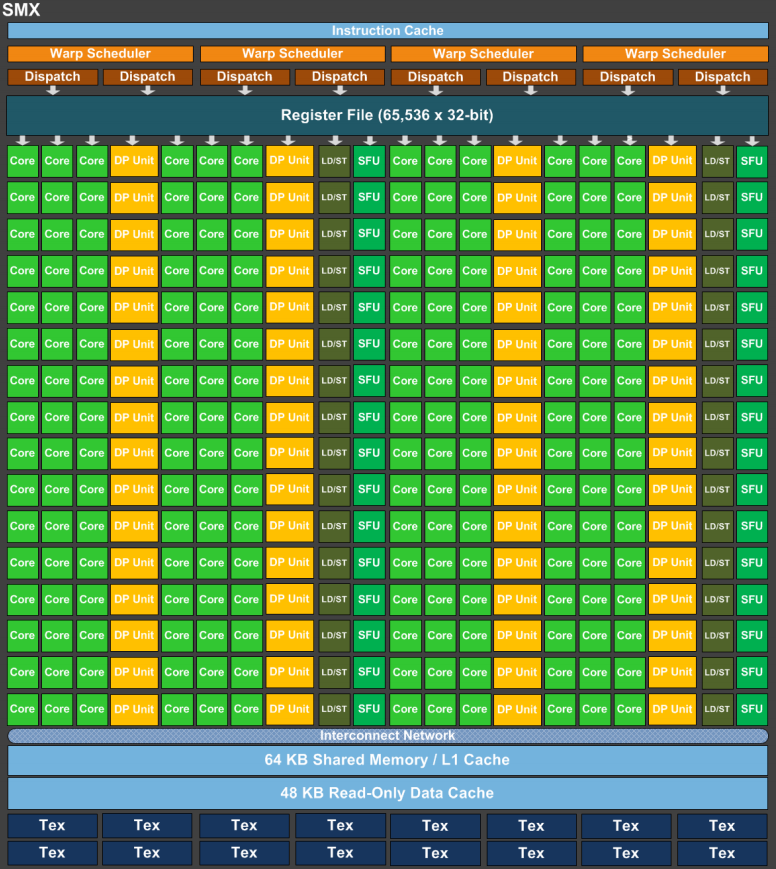
\includegraphics[width=0.7\textwidth]{./pics/2}
\caption{%
ساختار داخلی یک چندپردازنده جریانی در معماری
Kepler
}
\end{figure}

به لطف وجود چنین ظرفیت موازی‌سازی گسترده‌ای در پردازنده‌های گرافیکی زمان اجرای
محاسبات روی آن‌ها به شکل قابل توجهی کاهش می‌یابد. اما به دلایل مختلف 
مانند وابستگی‌داده‌ای بین دستورات، عدم قابلیت موازی‌سازی همه بخش‌های
پردازش، رفتار‌های مختلف
\LTRfootnote{Divergence}
 ریسه‌ها و در دستورات تصمیم‌گیری
\LTRfootnote{Decision Making}
و همچنین تاخیر‌های دسترسی به حافظه کارای پردازنده گرافیکی در شرایط واقعی بسیار
پایین‌تر از مقدار آن روی کاغذ است.

\section{ساختار پایان‌نامه}

در ادامه و پس از پایان مقدمه، در فصل دوم مفاهیم پایه‌ای در طراحی پردازنده‌های
چندهسته‌ای و به خصوص پردازنده‌های 
گرافیکی و به خصوص ساختاربندی حافظه در این تراشه‌ها را بررسی می‌کنیم. فصل سوم
مروری بر کارهای پیشین در موضوع پایان‌نامه خواهد بود. در فصل چهارم شهود و
انگیزه‌های اولیه برای این مطالعه را بررسی می‌کنم فصل پنجم را به معرفی
شبیه‌ساز و بررسی نتایج حاصل از شبیه‌سازی اختصاص می‌دهیم.
در
نهایت در فصل
ششم
به
جمع‌بندی و بررسی کارهای آتی می‌پردازیم.

% Chapter 2 %%%%%%%%%%%%%%%%%%%%%%%%%%%%%%%%%%%%%%%%%%%%%%

\chapter{
مفاهیم پایه‌
}

در این فصل ابتدا مروری کلی بر مفاهیم پردازنده‌های چند‌هسته‌ای و دلایل روی‌آوردن
به این پردازنده‌ها خواهیم داشت. در ادامه به بیان کلیاتی در مورد پردازنده‌های
گرافیکی و معماری و مدل برنامه‌سازی آن‌ها خواهیم پرداخت.

\section{
دلایل روی آوردن به پردازنده‌های چند‌هسته‌ای
}

زمانی که اندازه مشخصه
\LTRfootnote{Feature Size}
تزانزیستور‌ها با فاکتور
$k$
کاهش می‌یابد، به دلیل کوتاه‌تر شدن سیم‌ها و کاهش اندازه خازن در گیت‌ها
\LTRfootnote{Gate}
،
فرکانس کلاک
\LTRfootnote{Clock}
نیز با فاکتور
$k$
قابل افزایش است. همچنین تعداد ترانزیستور‌های موجود در واحد سطح با فاکتور
\lr{$x^2$}
و
اندازه قالب
\LTRfootnote{Die}
ترازیستور‌ها نیز با فاکتور
\lr{$k$}
قابل افزایش  می‌یابد. در چنین شرایطی قدرت پردازشی نیز به صورت تئوری با فاکتور
\lr{$k^4$}
افزایش  می‌یاد. هرچند در عمل به دلیل مواردی مانن توازی پنهان
\LTRfootnote{$Hidden Parallelism$}
 یا رفتار غیرقابل
پیش‌بینی حافظه نهان
\lr{$x^3$}
این فاکتور به طور عملی در مرتبه
\lr{$x^3$}
افزایش می‌یابد. به این نسبت‌ها قانون دانار گفته می‌شود
\LTRfootnote{Dannar Scaling (MOSFET Scaling)}
.
با این اوصاف به نظر می‌رسد که با معرفی هر نسل جدید پردازنده‌ها با اندازه مشخه
کوچکتر باید شاهد بهبود شگرف در عملکرد نرم‌افزارها باشیم. اما در عمل این رشد با
موانعی روبه‌روست که در ادامه به آن‌ها می‌پردازیم.

\begin{figure}[h]
\centering
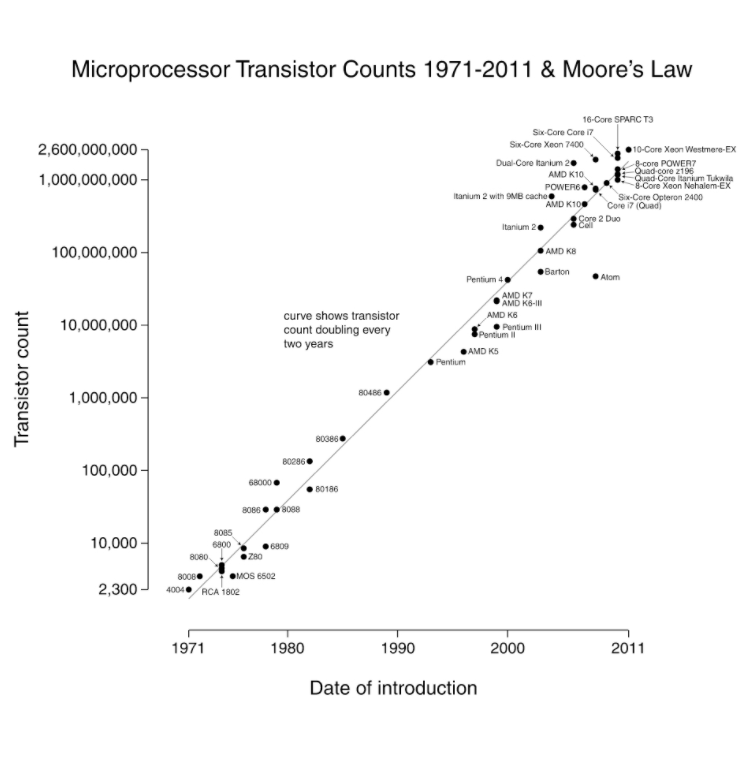
\includegraphics[width=\textwidth]{./pics/5}
\caption{تبعیت رشد تعداد ترانزیستور‌ها از قانون مور}
\label{moorelaw}
\end{figure}

\subsection{
چگالی توان
}

چگالی توان
\LTRfootnote{Power}
 به شکل میزان توان (نرخ انتقال انرژی) بر واحد حجم تعریف می‌شود. میزان
مصرف توان در تراشه‌ها به نرخ تغییر وضعیت گیت‌ها، یعنی نرخی که در آن 
خروجی یک گیت از صفر به یک تغییر می‌کند، بستگی‌دارد.
به
این
دلیل
به
اصطلاح گفته می‌شود که تراشه‌ها نرخ توان مصرفی پویا دارند.
با توجه به توضیح فوق انتظار می‌رود که نرخ توان مصرفی با افزایش فرکانس به طور
خطی افزایش پیدا کند. با توجه به افزایش نمایی فرکان پردازنده‌ها در سال‌های
پایانی دهه ۹۰ و اوایل قرن ۲۱ام، انتظار می‌رفت چگالی توان پردازنده‌ها در صورت
حفظ این نرخ رشد تا سال ۲۰۱۰ میلادی به ۱۰۰۰۰
وات بر سانتی‌متر مربع یعنی چیزی در حدود چگالی توان در سطح خورشید برسد. واضح است
که تراشه‌های نیمه رسانا در چنین وضعیتی تبخیر خواهند شد.

\subsection{
دیوار حافظه
}

به طور معمول هر دسترسی به حافظه اصلی
\LTRfootnote{Random Access Memory (RAM)}
در حدود صدها سیکل کلاک زمان می‌برد. به طور مثال پردازنده ممکن است برای اجرای
محاسبه‌ای که چند کلاک طول بکشد صدها کلاک منتظر دریافت داده و نوشتن مجدد آن در
حافظه بماند. به طور میانگین در سال‌های گذشته فرکانس حافظه هر 
شش سال دوبرابر می‌شد در حالی‌که که در تبیعت از قانون مور فرکانس پردازنده هر
دو سال دو برابر می‌شد. این تفاوت در نرخ رشد سبب ایجاد یک شکاف بزرگ میان عملکرد
پردازنده و حافظه می‌شود و حافظه را به گلوگاهی
\LTRfootnote{Bottleneck}
برای عملکرد سیستم تبدیل می‌کند و تاثیر افزایش فرکانس پردازنده را به شدت کاهش
می‌دهد. معماران سخت‌افزار با بهره‌گیری از ایده‌ها و روش‌های مختلف از جمله 
استفاده از چندین
لایه حافظه نهان و بهینه سازی‌هایی مانند 
\textit{%
بارگذاری با تاخیر
}
\LTRfootnote{Lazy Writeback}
و 
\textit{
کپی هنگام نوشتن
}
\LTRfootnote{Copy on Write}
سعی در مخفی کردن اثر سرعت حافظه از دید پردازنده دارند اما در نهایت مشکل همچنان
باقی است.
شکل
\ref{memorygap}
شکاف بین عملکرد پردازنده و حافظه اصلی را در سال‌های گذشته نشان می‌دهد.

\begin{figure}[h]
\centering
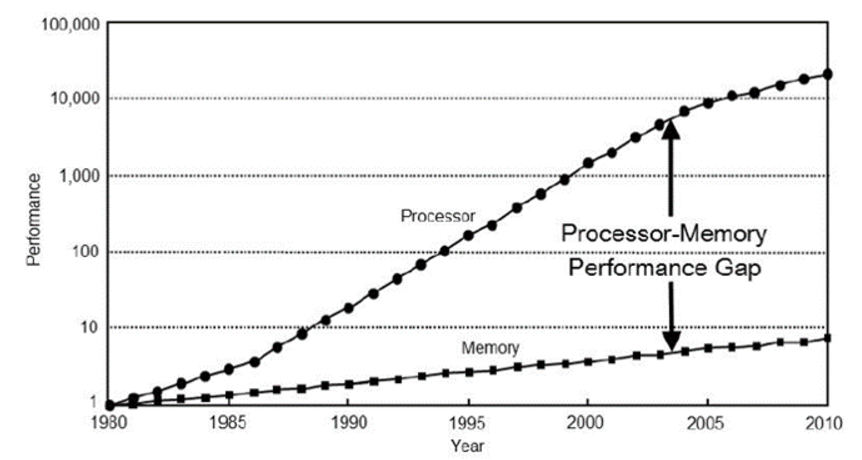
\includegraphics[width=\textwidth]{./pics/3}
\caption{شکاف بین عملکرد حافظه و پردازنده}
\label{memorygap}
\end{figure}

\begin{figure}[h]
\centering
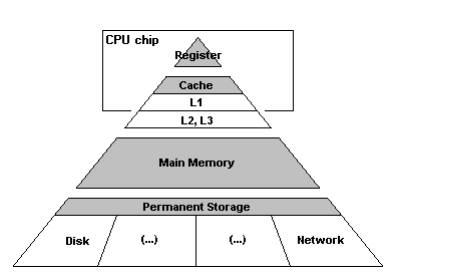
\includegraphics[width=\textwidth]{./pics/4}
\caption{سلسله مراتب حافظه در یک پردازنده امروزی}
\label{memoryhierarchy}
\end{figure}

\section{
پردازنده‌های چند‌هسته‌ای به عنوان یک راه‌حل
}

در زمانی که افزایش فرکانس پردازنده‌ها دیگر ممکن به نظر نمی‌رسد، مهندسان ایده
استفاده از چند پردازنده روی یک تراشه را برای بهبود عملکرد مطرح کردند. با توجه
به اینکه کارایی یک پردازنده با فرکانس کاری و تعداد هسته‌های آن متناسب است، با
افزایش تعداد هسته و ثابت نگه داشتن فرکانس می‌توانیم به عملکرد بهتری برسیم. با
پذیرفته شدن این معماری توسط تولید کنندگان مطرح مانند
Intel
و
AMD
از آن به بعد:

\begin{itemize}
\item 
چگالی ترانزیستو‌ر‌ها می‌تواند مانند قبل هر دو سال دو‌ برابر 
شود
\item
فرکانس پردازنده‌ها افزایش نمیابد (بعضا شاهد کاهش فرکانس برای ملاحظات توان مصرفی
هستیم)
\item
به جای دو برابر کردن فرکانس تمرکز روی دو برابر کردن تعداد هسته‌های پردازشی است
\end{itemize}


\section{
پردازنده‌های گرافیکی عام‌منظوره
}

به پردازنده‌های گرافیکی که قابلیت برنامه‌ریزی داشته باشد پردازنده گرافیکی
عام‌منظوره
\LTRfootnote{General Purpose Graphics Processing Unit}
گفته می‌شود. امروزه عمده کاربرد این پردازنده‌ها در محاسبات سنگین، شکستن رمز‌ها،
ارز‌های رمزنگاری‌شده
\LTRfootnote{Cryptocurrency}
و شبیه‌سازی‌های علمی است.

بر خلاف پردازنده‌های مرکزی که برای
اجرای سیستم عامل و
 سوییچ کردن
\LTRfootnote{Context Switching}
 بین تعداد زیادی پردازه
\LTRfootnote{Process}
اجرا و پنهان کردن تاخیر‌های حافظه برای حفظ پاسخگویی حداکثری طراحی شده‌اند،
پردازنده‌های گرافیکی با هدف حداکثر سرعت در محاسبات تولید می‌شوند و بسیاری از
پیچیدگی‌های داخلی پردازنده مرکزی را از معماری خود حذف می‌کنند. شکل
\ref{cpugpuperformancegap}
شکاف بین عملکرد این دو سخت‌افزار‌ را در محاسبات روی اعداد ممیز‌دار نشان می‌دهد.

\begin{figure}[h]
\centering
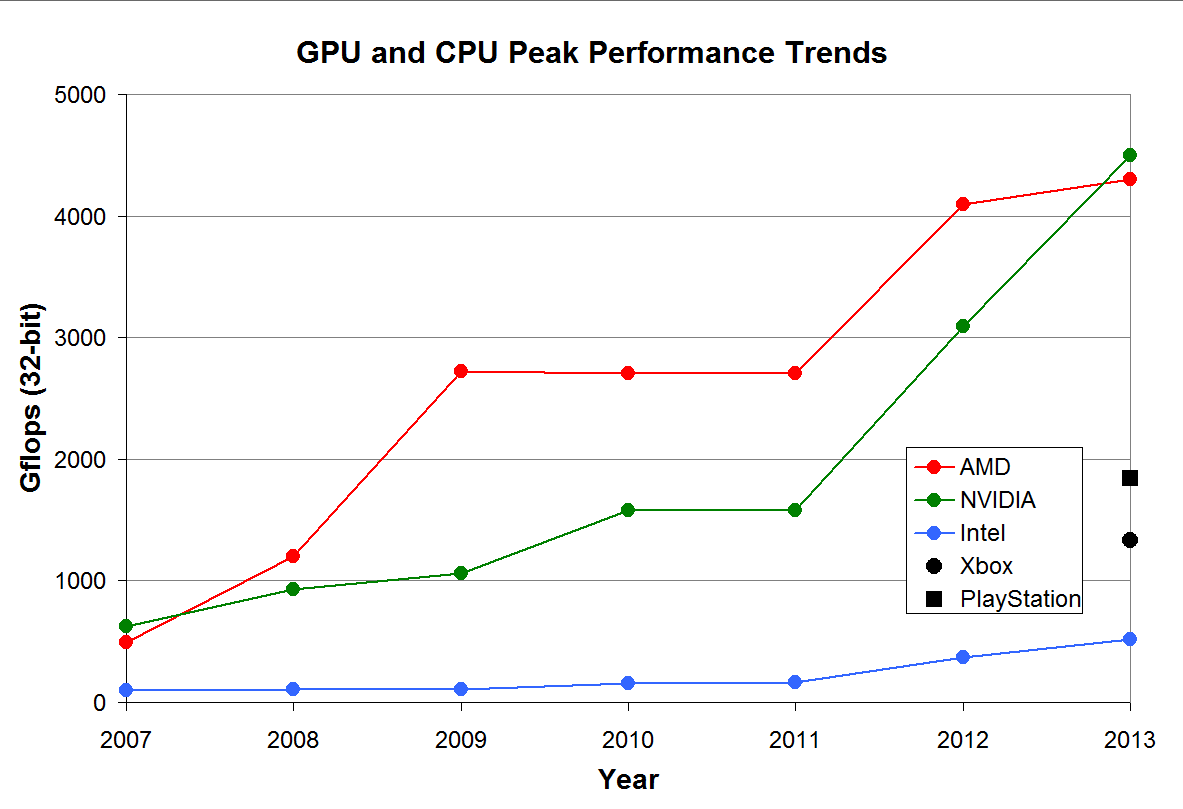
\includegraphics[width=\textwidth]{./pics/6}
\caption{شکاف بین عملکرد پردازنده مرکزی و پردازنده گرافیکی در محاسبات عددی}
\label{cpugpuperformancegap}
\end{figure}

\section{
استفاده از پردازنده گرافیکی برای مسائل عام‌منظوره
}


% Previous Works %%%%%%%%%%%%%%%%%%%%%%%%%%%%%%%%%%%%%%%%%
\chapter{
کارهای پیشین
}

% Motivation %%%%%%%%%%%%%%%%%%%%%%%%%%%%%%%%%%%%%%%%%%%%%
\chapter{
انگیزه و شهود
}

در این فصل ابتدا به بررسی وظایف حافظه مشترک و کاربرد‌های آن در پردازش‌های مختلف
می‌پردازیم و سپس روش‌های پیشنهادی خود را برای اندازه‌گیری عملکرد آن تحت بارهای
کاری علمی و نتایج به دست آمده را بررسی می‌کنیم.

در ادامه روشی برای بهبود عملکرد کلی تراشه گرافیک با تکیه بر تغییر معماری حافظه
مشترک پیشنهاد می‌دهیم و شهودی برای تاثیرگذار بودن این رویکرد ارائه می‌کنیم.

\section{
حافظه چرک‌نویس
}

حافظه چرک‌نویس 
\LTRfootnote{Scratchpad Memory}
به حافظه‌ای اطلاق می‌شود که نتایج میانی محاسبات را نگهداری می‌کند. 
scratchpad
معمولا نزدیک‌ترین واحد حافظه به
ALU
پس از رجیستر‌هاست و قادر به دسترسی مستقیم به حافظه اصلی
\LTRfootnote{Direct Memory Access (DMA)}
است. از آنجا که عمده نتایج میانی در محاسبات سنگین در پایان دور ریخته می‌شوند
استفاده از حافظه اصلی (و به تبع آن حافظه نهان) برای ذخیره‌سازی آن‌ها به علت
سرعت کم و نیز احتمال تاثیر منفی بر سایر دستورات در حال اجرا
(مصرف حافظه نهانی که می‌توانست به آن‌ها اختصاص پیدا کند) ضرورتی ندارد و در عوض
از یک حافظه سریع‌تر داخلی به این منظور استفاده می‌شود.

مزیت دیگر این واحد حافظه زمان دسترسی قابل پیش بینی به آن است، زیرا داده قبل از
رسیدن به پردازشگر از لایه‌های حافظه نهان عبور می‌کند و در زمان ثابتی قابل
دسترسی است.

\section{
حافظه مشترک
}

در پردازنده‌های مبتنی بر معماری کودا، به هر چندپردازنده‌ جریانی حافظه‌ای به
عنوان
\textit{%
حافظه مشترک
}
اختصاص داده می‌شود که عملا نقش همان چرک‌نویس را بازی می‌کند. برنامه‌نویس
می‌تواند از این حافظه برای ذخیره نتایج میانی و وضعیت فعلی پردازش و یا به عنوان
یک کپی سریع‌تر از حافظه اصلی استفاده کند. به عنوان مثال در معماری فرمی
\LTRfootnote{Fermi}
هر چندپردازنده دارای یک واحد حافظه ۶۴ کیلوبایتی است که بستگی به نیاز می‌تواند
۱۶ یا ۴۸ کیلوبایت از آن را در ابتدای اجرای کرنل به عنوان حافظه مشترک استفاده
کند.

\section{
شبیه‌ساز
\lr{GPGPU-Sim}
}

\lr{GPGPU-Sim}
یک شبیه‌ساز نوشته شده به زبان
\lr{C++}
برای شبیه‌سازی عملکرد پردازنده‌های گرافیکی 
است. با اینکه تاکید اصلی در طراحی این شبیه‌ساز برای مطابقت آن با معماری
CUDA
بوده است، اما این شبیه‌ساز به صورت داخلی از مدل انتزاعل قابل  انعطافی استفاده
می‌کند
که می‌تواند در صورت لزوم برای شبیه‌سازی سخت‌افزار‌های دیگر تولید‌کنندگان هم
مورد استفاده قرار بگیرد.
این شبیه‌ساز نرخ دستور بر کلاک
\LTRfootnote{Instructions Per Clock (IPC)}
تقریبا یکسان
(با همبستگی حدود ۹۸ درصد با سخت‌افزار کودا) نشان می‌دهد و به از این جهت برای
سنجش عملکر پردازنده گرافیکی بسیار مناسب به نظر می‌رسد.
شکل
\ref{ipccorrelation}
این رفتار شبیه‌ساز را نشان می‌دهد
.
 بحث بیشتر در مورد جزییات داخلی این شبیه‌ساز خارج از
حوصله این نوشتار است.

\begin{figure}[h]
\centering
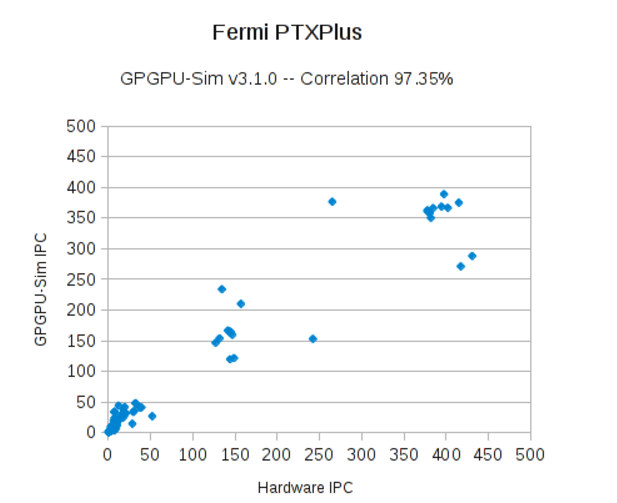
\includegraphics[width=\textwidth]{./pics/7}
\caption{همبستگی نرخ 
IPC
میان شبیه‌ساز و سخت‌افزار نسل
Fermi
}
\label{ipccorrelation}
\end{figure}

\section{
بررسی کاربرد حافظه مشترک در محاسبات عام‌منظوره
}

در طول این مطالعه برای بررسی عملکر حافظه مشترک از ۳ مجموعه بنچمارک
\LTRfootnote{Benchmark{
استفاده شده است:
\begin{enumerate}
\item 
مجموعه
بنچمارک
رودینیا
\LTRfootnote{Rodinia}
دانشگاه ویرجینا
\item
مجموعه بنچمارک
پاربویل
\LTRfootnote{Parboil}
دانشگاه
ایلینویز
\item
مجموعه بنچمارک
ISPASS
\end{enumerate}

این بنچمارک‌ها مجموعه‌ای از الگوریتم‌های رایج در حوزه‌های مختلف علمی و مهندسی
را پوشش می‌دهند

\begin{center}
\begin{table}
\begin{tabular}{|l|l|l|}
\begin{latin}
\hline
BFS & Breadth-First Search & Graph \\
\hline
CUTCP & Distance-Cutoff Coulombic Potential & Molecular Simulation \\
\hline
HISTO & Saturating Histogram & Statistics \\
\hline
LBM & Lattice-Boltzmann Method & Fluid Dynamics \\
\hline
MM & Dense Matrix-Matrix Multiply & Linear Algebra \\
\hline
MRI-GRIDDING & Magnteic Resonance Imaging - Gridding & Medical Imaging\\
\hline
MRI-Q & Magnetic Resonance Imaging - Q & Medical Imaging \\
\hline
SAD & Sum of Absolute Differences & MPEG video encoding \\
\hline
PMV & Sparse-Matrix Dense-Vector Multiplication & Linear Algebra \\
\hline
STENCIL & 3-D Stencil Operation & Graphics \\
\hline
TPACF & Two Point Angular Correlation Function & Atronomy \\
\hline
\end{latin}
\end{tabular}	
\caption{گستره بنچمارک‌های موجود در پکیج پاربویل}
\label{table:parboilbenchmarks}
\end{table}
\end{center}


% Bibliography %%%%%%%%%%%%%%%%%%%%%%%%%%%%%%%%%%%%%%%%%%%
\PrepareForBiblio
\begin{thebibliography}{1}
\begin{LTRitems}

\setpersianfont\bibitem{parsilatex}\resetlatinfont
\newblock S. Borkar, {\itshape``Design challenges of technology scaling''} in
IEEE Micro,
vol.
19,
no. 4, pp. 23-29, Jul-Aug 1999.

\setpersianfont\bibitem{parsilatex}\resetlatinfont
\newblock M. D. Hill and M. R. Marty, {\itshape``Amdahl's Law in the Multicore
Era,''} in
Computer,
vol. 41, no. 7, pp. 33-38, July 2008.

\setpersianfont\bibitem{parsilatex}\resetlatinfont
\newblock Nvidia Corportaion, {\itshape``
\href{https://www.nvidia.com/content/PDF/kepler/NVIDIA-Kepler
-GK110-Architecture-Whitepaper.pdf}{Nvidia Kepler GK110 Architecture
Whitepaper}}''


\setpersianfont\bibitem{parsilatex}\resetlatinfont
\newblock R. H. Dennard, F. H. Gaensslen, V. L. Rideout, E. Bassous and A. R.
LeBlanc, {\itshape``Design of ion-implanted MOSFET's with very small physical
dimensions,''} in IEEE Journal of Solid-State Circuits, vol. 9, no. 5, pp.
256-268, Oct 1974.

\setpersianfont\bibitem{parsilatex}\resetlatinfont
\newblock D. Luebke, {\itshape ``CUDA: Scalable parallel programming for
high-performance
scientific
computing''}, 2008 5th IEEE International Symposium on Biomedical Imaging: From
Nano to Macro, Paris, 2008, pp. 836-838.

\setpersianfont\bibitem{parsilatex}\resetlatinfont
\newblockTyler Sorensen, Ganesh Gopalakrishnan, and Vinod Grover. 2013.
{\itshape ``Towards
shared
memory consistency models for GPUs''}. In Proceedings of the 27th international
ACM conference on International conference on supercomputing (ICS '13)

\setpersianfont\bibitem{parsilatex}\resetlatinfont
\newblock A. Bakhoda, G. L. Yuan, W. W. L. Fung, H. Wong and T. M. Aamodt,
{\itshape ``Analyzing
CUDA workloads using a detailed GPU simulator," 2009 IEEE International
Symposium on Performance Analysis of Systems and Software, Boston''}, MA, 2009,
pp. 163-174.

\setpersianfont\bibitem{parsilatex}\resetlatinfont
\newblock S. Che et al., {\itshape ``Rodinia: A benchmark suite for
heterogeneous
computing,''} 2009
IEEE International Symposium on Workload Characterization (IISWC), Austin, TX,
2009, pp. 44-54.

\setpersianfont\bibitem{parsilatex}\resetlatinfont
\newblock Stratton, John A., et al. {\itshape ``Parboil: A revised benchmark
suite
for
scientific
and commercial throughput computing.''} Center for Reliable and
High-Performance
Computing 127 (2012).

\end{LTRitems}

\end{thebibliography}
%%%%%%%%%%%%%%%%%%%%%%%%%%%%%%%%%%%%%%%%%%%%%%%%%%%%%%%%%%
\PrepareForLatinPages
\date{October 6, 2011}
\title{\sffamily Thesis Class in XeLaTeX}
\author{\sffamily Mohsen SHARIFI TABAR}
\university{Sharif University of Technology\\Department of Mathematical
Sciences}
\subject{Pure Mathematics}
\supervisor{\sffamily Dr. Supervisor}
\consult{\sffamily Dr. Consult}
\begin{abstract}{first latin keyword, second latin keyword, third latin
keyword.}
There is no special abstract for this thesis.
\end{abstract}
\makethesistitle
\end{document}